\chapter{Síntesis de Sonidos mediante Modelos Físicos}

\section{Introducción}
Se utilizó el modelo de Karplus-Strong para sintetizar el sonido de instrumentos de cuerda percutida u otros tipos de percusión. Este algoritmo, creado por Kevin Karplus y Alexander Strong en 1983 para sintetizar sonidos con pocos recursos y a tiempo real.

En este trabajo se analizaron el modelo básico para la síntesis de cuerdas percutidas y el modelo modificado para la síntesis de instrumentos de percusión.

\section{Modelo Conceptual}

En principio, el sistema se trata de un sistema linear excitado con una secuencia aleatoria de longitud finita $L$. El sistema consiste de una linea de retardo de $L$ muestras realimentadas a travéz de un filtro, tal como se ve en la figura \ref{fig:KS_model}.

\begin{figure}[ht]
    \centering
    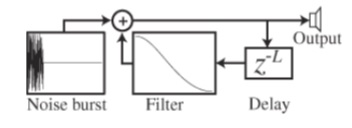
\includegraphics{res/ks_concept.jpg}
    \caption{Diagrama Conceptual del Modelo de Karplus-Strong}
    \label{fig:KS_model}
\end{figure}

La línea de retardo simula la cuerda, la cual los distintos armónicos de una nota recorren, se atenúan y decaen en el tiempo. En el modelo principal que se plantea en trabajo original de Kevin Karplus y Alex Strong, a la ausencia de algún filtro a la salida de la línea de retardo, la salida del sistema sería una repetición periódica de la señal entrante, lo que generaría un tono puro con una frecuencia de $f_s / L$, donde $f_s$ es la frecuencia de sampleo del sistema.

La modificación que inventa Alex Strong es promediar dos muestras consecutivas del sistema, generando un decaimiento lento de la amplitud en el tiempo. Matemáticamente, esta operación puede expresarse como en la expresión \eqref{eq:KS_avg}.

\begin{equation}
    Y_t = 0.5\times \left(Y_{t-L}+Y_{t-L-1}\right)
    \label{eq:KS_avg}
\end{equation}

Como consecuencia de esta modificación, la frecuencia del tono generado estará dada por la expresión \eqref{eq:KS_pitch}. Este tono tiene un sonido similar al de una cuerta percutida. Independientemente de las condiciones iniciales del sistema, el espectro decaerá hacia un tono puro, y eventualmente, a un valor constante (el silencio)

\begin{equation}
    f = \frac{f_s}{L+1/2}
    \label{eq:KS_pitch}
\end{equation}

Dado que para producir un sonido realista, se desea que el impulso inicial del sistema contenga una gran variedad de armónicos. Para ello existen distintas opciones. La primera es la propuesta por el mismo trabajo de Karplus-Strong: una señal aleatoria bi-nivel cuya expresión matemática está dada por \eqref{eq:2_level_random}, donde $A$ es la amplitud de la nota. Otras opciones para la excitación inicial con ruido es utilizar señales de ruido con distribución uniforme o gaussiana. Como estas muestras iniciales son repetidas periódicamente, no generarán ruido en el fondo.

\begin{equation}
    Y_t = 
    \begin{cases}
        +A  &   \text{probabilidad 0.5}\\
        -A  &   \text{probabilidad 0.5}
    \end{cases}
    \qquad  \text{para} -L\leq t \leq 0
    \label{eq:2_level_random}
\end{equation}

Finalemente, el modelo utilizado para simular la cuerda percutida será el de la figura \ref{fig:ks_original}. $x(n)$ será la señal inicial de entrada, por donde entrará la señal de ruido de longitud de muestras $L$.

\begin{figure}[ht]
    \centering
    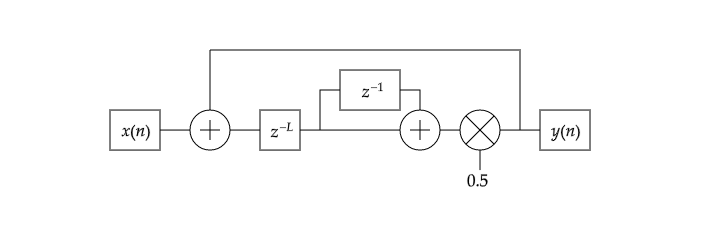
\includegraphics[width = \linewidth]{res/fig_ks.png}
    \caption{Modelo Original de Karplus Strong}
    \label{fig:ks_original}
\end{figure}

Modificando el modelo también es posible sintetizar instrumentos de percusión. Si se cambia el signo del promedio de las muestras aleatoriamente, como se ve en la figura \ref{fig:ks_drum}, matemáticamente tendrá un comportamiento expresado en \eqref{eq:ks_drum}. $b$ es llamado el factor de mezcla. Cuando $b=1$, el sistema se comporta normalmente y sigue simulando una cuerda. Cuando $b=0$, la señal es negada cada $L+0.5$ muestras, generando un sonido parecido a un arpa.

Finalemente, cuando $b=0.5$ se pierde el "tono" del sonido y este se asemejará más a un sonido percutido. $L$ ya no controla el tono, sino el tiempo de decaimiento. Dado que la naturaleza aleatoria ya se encuentra dentro del sistema, es suficiente con inicializar el sistema con una señal constante en lugar de utilizar ruido.

\begin{figure}[ht]
    \centering
    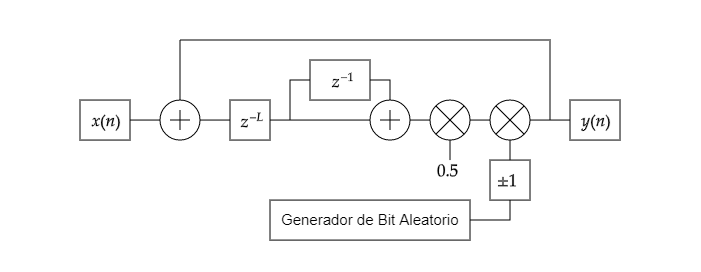
\includegraphics[width = \linewidth]{res/fig_ks_drum.png}
    \caption{Modelo Modificado de Karplus Strong para instrumentos de percusión}
    \label{fig:ks_drum}
\end{figure}

\begin{equation}
    Y_t = 
    \begin{cases}
        0.5\times \left(Y_{t-L}+Y_{t-L-1}\right) &   \text{probabilidad} \quad b \\
        -0.5\times \left(Y_{t-L}+Y_{t-L-1}\right) &   \text{probabilidad} \quad 1-b
    \end{cases}
    \label{eq:ks_drum}
\end{equation}

\section{Transferencia del Modelo}

Se calculó la función transferencia del modelo original de Karplus-Strong.

La transferencia del promedio está dada por

\begin{equation}
    H_a(z) = \frac{1+z^{-1}}{2}
\end{equation}

y la transferencia de la línea de retardo está dada por

\begin{equation}
    H_b(z) = z^{-L}
\end{equation}

Con esto, se obtiene que la transferencia de todo el sistema está dada por

\begin{equation}
    H(z) = \frac{1}{1- H_a(z) H_b(z)} = \frac{1/2\cdot (1+z^{-1})}{1-1/2\cdot z^{-L}(1+z^{-1})}= \frac{z+1}{2z^{L+1}-z-1}
    \label{eq:KS_H}
\end{equation}

A partir de la expresión \eqref{eq:KS_H} se puede calcular que existe un único cero en $z=-1$, que corresponde a la frecuencia de Nyquist $f_s/2$. Los polos pueden ser encontrados calculando las raíces de la expresión $2z^{L+1}-z-1 = 0$. Estas se pueden aproximar si la expresamos de la forma $2z^{L+1/2} = z^{1/2} + z^{-1/2}$. Reemplazando $z=a e^{j\omega}$ se obtiene:

\begin{equation}
    2 a^{L+1/2} e^{j\omega(L+1/2)} = a^{1/2}e^{j\omega/2} + a^{-1/2}e^{-j\omega/2}=\sqrt{a + a^{-1} + 2 \cos\omega } \cdot e^{j\theta}
\end{equation}

Analizando las partes imaginarias, se obtiene que

\begin{equation*}
    \sqrt{a + a^{-1} + 2 \cos\omega } \sin\theta = (a^{1/2} - a^{-1/2}) \sin\frac{\omega}{2}
\end{equation*}

Aproximando $e^{j\omega(L+1/2)} \approx 1$ se despeja que $\omega = 2 \pi n / (L+1/2)$. Aproximando $2 a^{p+1/2}\approx 2 cos(\omega/2)$ se puede despejar la constante del tiempo de caída del n-ésimo armónico, siendo
\begin{equation}
    a=\left[\cos\left( \frac{2 \pi n}{2L+1}\right)\right]^{1/(L+1/2)} = \left[\cos\left( \pi n \frac{f}{f_s}\right) \right]^{f/f_s}
\end{equation}

Por lo tanto, los polos estarán ubicados en $z = a e^{j\omega}$ donde

\begin{equation*}
    a = \left[\cos\left( \frac{2 \pi n}{2L+1}\right)\right]^{1/(L+1/2)} \qquad \omega = \frac{2 \pi n}{L+1/2}
\end{equation*}

